\chapter{Creating a Quantified Yolngu Calendar}
\label{ch:quantify}
The mixed methods, results, and interpretive discussion.

\section{Methods}

\emph{TODO:  expand section}
\begin{itemize}
\item Briefly describe interview technique to elicit details, how coded in transcripts/notes
\item Touch on literature for seasonal onset detection (eg monsoon).
        Stats with time series and missing data are also relevant.
\item Three approaches minimum:  traditional, and others discussed with SCU
\item Describe statistical approaches and meta-method for using them all
\item Outline how to select, normalise, check input data (eg comparison across stations)
\end{itemize}

\begin{figure}[h]
    \centering
    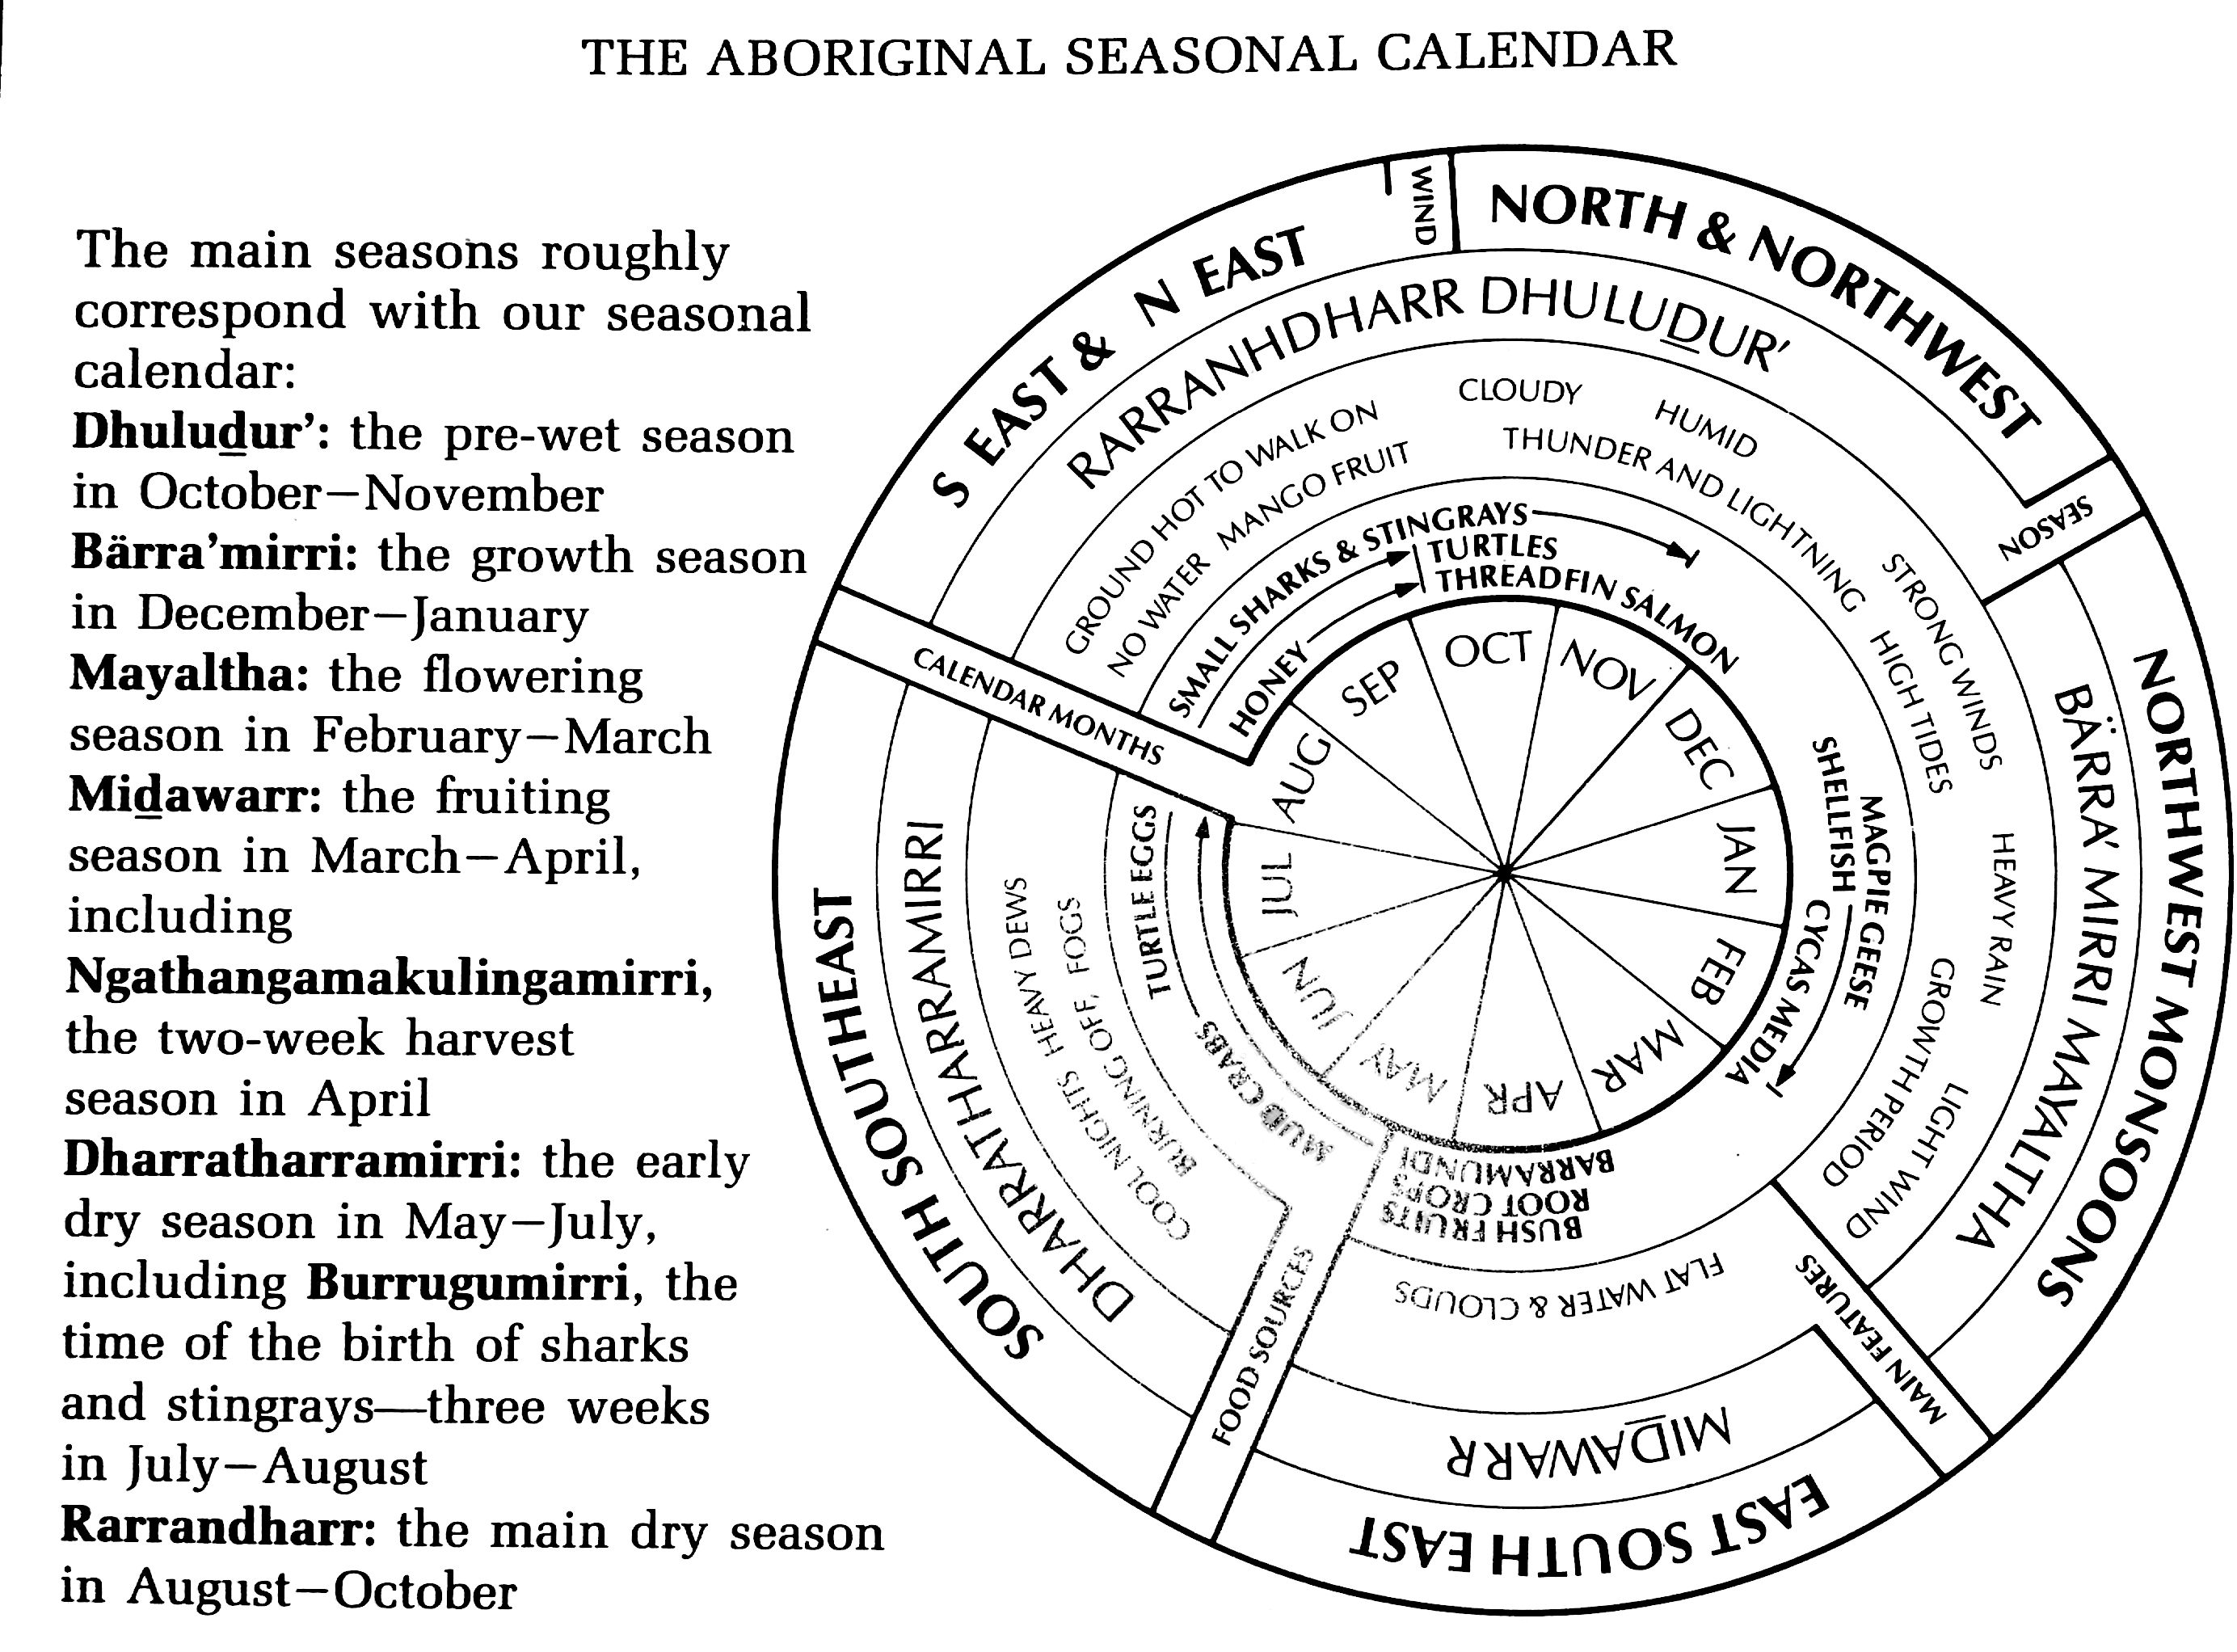
\includegraphics[width=\textwidth]{yolngu-calendar.jpg}
    \caption{Conceptual Yolngu seasonal calendar \citep{davis1989}}
    \label{fig:yolngu-seasons}
\end{figure}

\section{Results and Discussion}

\begin{enumerate}
\item The six seasons are XXX (see above).  They are defined by XXX.
        This calendar has the following interesting properties:
        (eg – variable onset, multiple occurrence, at-least-once by climate not construction).
\item Summary statistics (as charts) for input data, ie weather observations.
\item For each season:
\item Determine seasons by each approach, and discuss reliability
\item APPROACH is best, for REASONS.  Finer distinctions if applicable.
\item The Quantified calendar is as follows:  XXX (with detection functions)
\end{enumerate}

\begin{figure}[p]
    \centering
    \includegraphics[width=\textwidth]{galiwinku-all.pdf}
    \caption[Historical weather observations at Elcho Island]{
        Historical weather observations at Elcho Island.  Each panel shows a single variable, with years on the y axis and day-of-year on the x.
        Note that each variable has a different seasonal pattern, and that seasonality changes from year to year.}
    \label{fig:galiwinku-observations}
\end{figure}
% Note - if possible, these figures should be on facing pages to allow easy comparison
\begin{figure}[p]
    \centering
    \includegraphics[width=\textwidth]{milingimbi-all.pdf}
    \caption[Historical weather observations at Milingimbi Airport]{
        Historical weather observations at Milingimbi Airport.  Each panel shows a single variable, with years on the y axis and day-of-year on the x.
        Note that each variable has a different seasonal pattern, and that seasonality changes from year to year.}
    \label{fig:milingimbi-observations}
\end{figure}

\begin{landscape}
\begin{table}
    \input{../output/galiwinku-summary-table.tex}
    \caption{Monthly mean weather observations at Galiwinku}
    \label{tab:galiwinku-DRAFT-ONLY}
\end{table}
\end{landscape}

